\documentclass[a4paper, 12pt]{report}
\usepackage[left=2.5cm, right=2.5cm, top=3cm, bottom=3cm]{geometry}

\usepackage{xcolor}
\usepackage{amsmath, amssymb, amsfonts, amsthm}
\usepackage{url}
\usepackage{graphicx}

% use spanish template
% \usepackage[spanish]{babel}

% add bibliographics quotes
\usepackage{cite}

% insert source code in latex
\usepackage{listings}
\usepackage{color}

\definecolor{gray97}{gray}{.97}
\definecolor{gray75}{gray}{.75}
\definecolor{gray45}{gray}{.45}
\lstset{
  frame=Ltb,
  framerule=0pt,
  aboveskip=0.5cm,
  framextopmargin=3pt,
  framexleftmargin=0.4cm,
  framesep=0pt,
  rulesep=.4pt,
  backgroundcolor=\color{gray97},
  rulesepcolor=\color{white},
  %
  showstringspaces=true, columns=fullflexible, basicstyle=\ttfamily,
  stringstyle=\color{orange}, commentstyle=\color{gray45},
  keywordstyle=\bfseries\color{green!40!white},
  %
  numbers=left, numbersep=15pt, numberstyle=\tiny, numberfirstline=false,
  breaklines=true,
}

\lstnewenvironment{listing}[1][]
{\lstset{#1}\pagebreak[0]}{\pagebreak[0]}

\begin{document}
\title{\bf HULK Interpreter Project }
\author{Mauricio Sunde Jimenez C111}
\date{\today}
\maketitle

\begin{abstract}
    Un Intérprete es un programa informático que ejecuta directamente instrucciones escritas en un lenguaje de programación o scripting, sin necesidad de que hayan sido compiladas previamente en un programa en lenguaje de máquina.

    HULK es un lenguaje de programación orientado a objetos, con herencia simple, polimorfismo y encapsulación a nivel de clase. Además, en HULK es posible definir funciones globales fuera del alcance de todas las clases. También es posible definir una única expresión global que constituya el punto de entrada al programa. Pero para este proyecto haremos un subconjunto de HULK. 
\end{abstract}

\tableofcontents

\newpage

\section*{Contexto}
\addcontentsline{toc}{section}{\bf Contexto}

Es un lenguaje de programación imperativo, funcional, estática y fuertemente tipado. Casi todas las instrucciones en HULK son expresiones. En particular, el subconjunto de HULK que se implemento se compone solamente de expresiones que pueden escribirse en una línea.

\subsection*{HulkExpressions}
\addcontentsline{toc}{subsection}{HulkExpressions}

En HULK la mayoría de las construcciones sintácticas son expresiones,
incluido el cuerpo de todas las funciones y otros. El cuerpo de un programa en HULK siempre termina con un unico punto y coma.

Este es un ejemplo de una posible entrada.

\begin{lstlisting}
print("Hello world!");
\end{lstlisting}

La entrada mas clasica de todo lenguaje de programacion. Aqui print es una funcion que recibe un argumento e imprime en consola el resultado.

\subsubsection*{Hulk Arithmetic Operations}
\addcontentsline{toc}{subsubsection}{Arithmetic operations}

HULK define tipos de literales como numbers, strings y booleanos. Hulk admite cualquier expression matematica entre numeros, tales como suma, resta, multipicacion, division, exponenciacion etc. Siempre y cuando sean del mismo tipo las expresiones.

Este seria un ejemplo de expresion correcta.

\begin{lstlisting}
print(2 + 3);
\end{lstlisting}

\subsubsection*{Hulk Strings}
\addcontentsline{toc}{subsubsection}{Hulk Strings}

Los strings en Hulk estan definidos como una cadena de caracteres que comienza y termina con Comillas.
Como por ejemplo;
\begin{lstlisting}
"Hulk is Fun"
\end{lstlisting}

Tambien podemos concatenar strings con el operador @.

\begin{lstlisting}
print("Hulk" @ " " @ "is" @ " " @ "Fun");
\end{lstlisting}

\subsubsection*{Standard Library of Functions}

Tenemos ademas de las funciones inline que se crean durante el tiempo de ejectucion, la biblioteca de funciones aritmeticas siguientes.

\begin{itemize}
  \item {\tt sqrt(<value>)} Evalua la raiz cuadrada de dicho valor.
  \item {\tt sin{<angle>}}  Evalua el seno del valor.
  \item {\tt cos(<angle>)} Evalua el coseno del valor.
  \item {\tt log(<base>, <value>)} Evalua el logaritmo del valor en una base definida por el usuario.
\end{itemize}

Ademas de estas funciones tenemos tambien las variables globales PI y E las cuales son la representacion matematica de dichos valores.
Este seria un programa valido.
\begin{lstlisting}
print(PI + E + cos(PI / 2));
\end{lstlisting}

\subsection*{Hulk Functions}
\addcontentsline{toc}{subsection}{Hulk Functions}

En HULK hay dos tipos de funciones, las funciones inline y las funciones regulares. En este proyecto solo se implementan las funciones inline. Una vez definida una función, puede usarse en una expresión cualquiera. El cuerpo de una función inline es una expresión cualquiera, que por supuesto puede incluir otras funciones y expresiones básicas, o cualquier combinación.

\subsubsection*{Hulk Inline functions}
\addcontentsline{toc}{subsubsection}{Hulk Inline functions}
En Hulk podemos definir una funcion de la siguiente forma.
\begin{lstlisting}
function tan(x) => sin(x) / cos(x);
\end{lstlisting}

Una función en línea se define mediante un identificador seguido de argumentos entre paréntesis,separados por coma en caso de ser mas de uno,
luego el símbolo =>, y luego una expresión y siempre
terminando con un punto y coma final.

Este subconjunto de Hulk tambien permite Funciones recursivas (Brutal!!).
\begin{lstlisting}
function fact(x) => if (x == 1) 1 else x * fact(x - 1)
\end{lstlisting}

\subsection*{Hulk Let in Declarations}
\addcontentsline{toc}{subsection}{Let in Variables}

Las variables en HULK tienen un tiempo de vida, lo que significa que solo viven dentro de su inExpression es decir despuues de ser declaradas con let. 
La expresión let se utiliza para introducir una o más variables y evaluar una expresión en
un nuevo alcance donde se definen las variables.

Aqui se declara una variable a que solo existe en el cuerpo del in.
\begin{lstlisting}
let a = 2 in print(a);
\end{lstlisting}
En este ejemplo el in mas externo no reconocera a b ya que su scope fue utilizado anteriormente y la variable deja de existir.
\begin{lstlisting}
    let a = 2 in let b = 2 in b in a + b;
\end{lstlisting}

Tambien podemos definir multiples variables con un solo let.
Dado que el scoping del let se realiza de izquierda a derecha, y cada
variable está efectivamente vinculada en un nuevo scope, puede usar con seguridad una variable al definir otra como en este caso el in del let reconoce a todas las variables.
\begin{lstlisting}
let a = 2, b = 3, c = 4 ... in ...;
\end{lstlisting}


\begin{lstlisting}
let a = 1, b = a in print(b);
\end{lstlisting}

Pero tambien es valido.
\begin{lstlisting}
let a = 1 in let b = a in print(b);
\end{lstlisting}
El valor de retorno de cada LetInExpression esta dado por el valor de su cuerpo.

En HULK, cada nuevo scope oculta los símbolos del scope principal, lo que significa que puede redefinir el nombre de una variable.
en una expresión interna del let tal como:

\begin{lstlisting}
let a = 2, a = 3 , a =4 ... in print (a);
\end{lstlisting}
O tambien.
\begin{lstlisting}
    let a = 2 in let a = 4 in let a = 3 in print (a);
\end{lstlisting}


\subsection*{Hulk IfElse}
\addcontentsline{toc}{subsection}{HulkIfElse}

Las condiciones en HULK se implementan con la expresión if-else, que recibe una expresión booleana entre paréntesis, y dos expresiones para el cuerpo del if y el else respectivamente. Siempre deben incluirse ambas partes:

\begin{lstlisting}
let a = 42 in if (a % 2 == 0) print("Even") else print("Odd");
\end{lstlisting}

Como ifElse es una expresión, se puede usar dentro de otra expresión al estilo del operador ternario en CSharp.

\begin{lstlisting}
let a = 42 in print(if(a % 2 == 0) "Even" else "Odd");
\end{lstlisting}


\subsection*{Hulk Errors}
\addcontentsline{toc}{subsection}{Hulk Errors}

En HULK hay 3 tipos de errores que usted debe detectar. En caso de detectarse un error, el intérprete debe imprimir una línea indicando el error que sea lo más informativa posible.

\subsubsection*{Lexical Error}
\addcontentsline{toc}{subsubsection}{Lexical Error}

Errores que se producen por la presencia de tokens inválidos. Por ejemplo:

\begin{lstlisting}
    let 14a = 5 in print(14a); 
    ! LEXICAL ERROR: `14a` is not valid token.
\end{lstlisting}

\subsubsection*{Syntax Error}
\addcontentsline{toc}{subsubsection}{Syntax Error}

Errores que se producen por expresiones mal formadas como paréntesis no balanceados o expresiones incompletas. Por ejemplo:

\begin{lstlisting}
    > let a = 5 in print(a;
    ! SYNTAX ERROR: Missing closing parenthesis after `a`.
    > let a = 5 inn print(a);
    ! SYNTAX ERROR: Invalid token `inn` in `let-in` expression.
    > let a = in print(a);
    ! SYNTAX ERROR: Missing expression in `let-in` after variable `a`.
\end{lstlisting}

\subsubsection*{Semantic Error}
\addcontentsline{toc}{subsubsection}{Semantic Error}

Errores que se producen por el uso incorrecto de los tipos y argumentos. Por ejemplo:

\begin{lstlisting}
    > let a = "hello world" in print(a + 5);
    ! SEMANTIC ERROR: Operator `+` cannot be used between `string` and `number`.
    > print(fib("hello world"));
    ! SEMANTIC ERROR: Function `fib` receives `number`, not `string`.
    > print(fib(4,3));
    ! SEMANTIC ERROR: Function `fib` receives 1 argument(s), but 2 were given.
\end{lstlisting}

\section*{Implementaciones}
\addcontentsline{toc}{section}{\bf Proceso del Interpreter}
Aqui se llevara a cabo un poco de como funciona el interprete.

\subsection*{Lexical Analysis}
\addcontentsline{toc}{subsection}{Lexer}

El primer paso en el intérprete es analizar el texto de entrada. El lexer toma el texto sin formato como una serie de caracteres. Despues los examina y los distribuye en una lista de tokens es decir palabras reconocidas por el lenguaje

En primer lugar, necesitamos identificar todos los tipos de tokens que se utilizan en la gramática del idioma. Algunos de estos tipos son:

Los Operadores como *,+,=,-,/,@,Modulo. 
Caracteres como el punto(.), la coma(,), el punto y coma(;), los parentesis ( , ).
Los Operadores de comparacion >=,==,<=,!=,=,>,<,.
Los literales como los numeros, strings, booleanos, o identificadores.
Las keyWords del lenguaje como AND,OR,False,True,Function,If,Else,Let,In.


En el proceso de lexing se utilizo expresiones regulares. Las expresiones regulares son patrones utilizados para encontrar una determinada combinación de caracteres dentro de una cadena de texto. Las expresiones regulares proporcionan una manera muy flexible de buscar o reconocer cadenas de texto. Una vez con dichos patrones se revisa si existe algun match y de ser asi se revisa el tipo de token al que pertenece, por ejemplo:

\begin{figure}[h]
    \center
    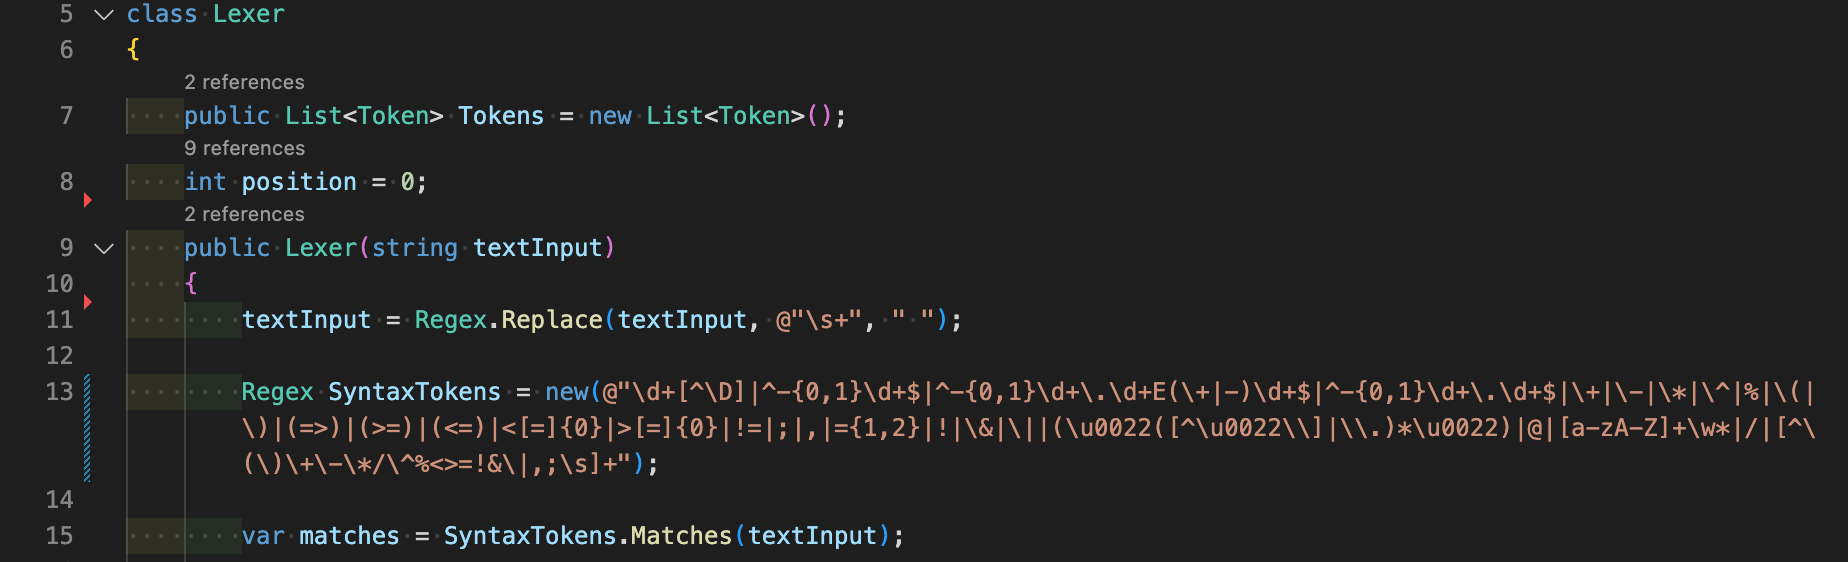
\includegraphics[width=10cm]{Pictures For Hulk/Figure1.png}
    \caption{Muestra del Patron de regex}
    \label{fig:logo}
\end{figure}

\begin{figure}[h]
    \center
    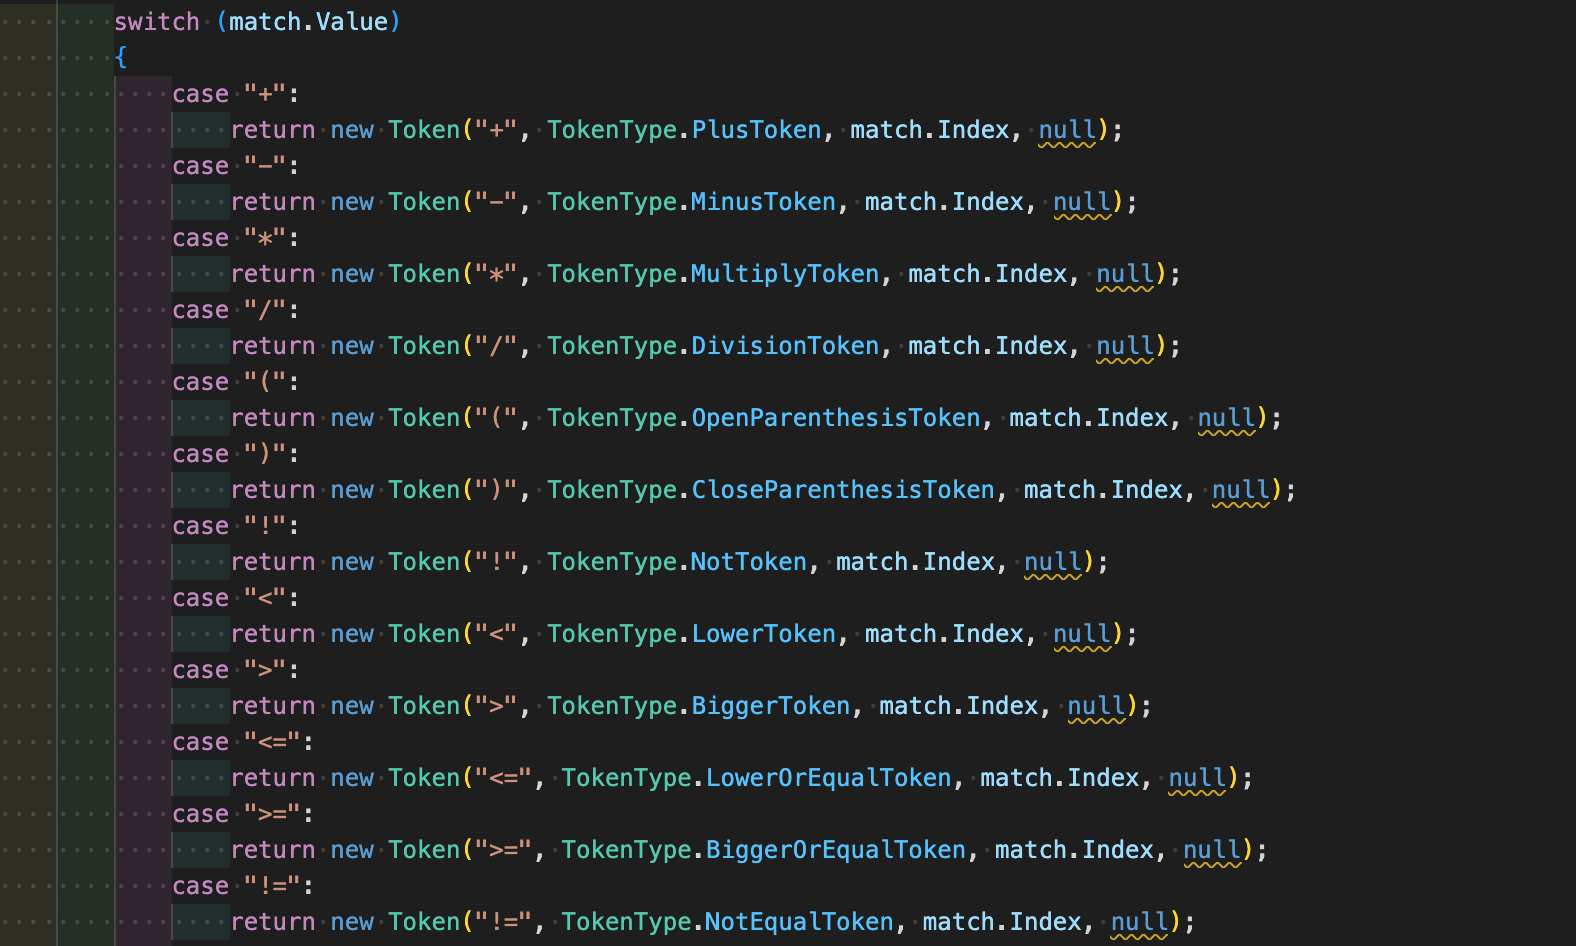
\includegraphics[width=10cm]{Pictures For Hulk/Figure2.png}
    \caption{Muestra de distintos matches y asignandole el tipo de token}
    \label{fig:logo}
\end{figure}

\begin{figure}[h]
    \center
    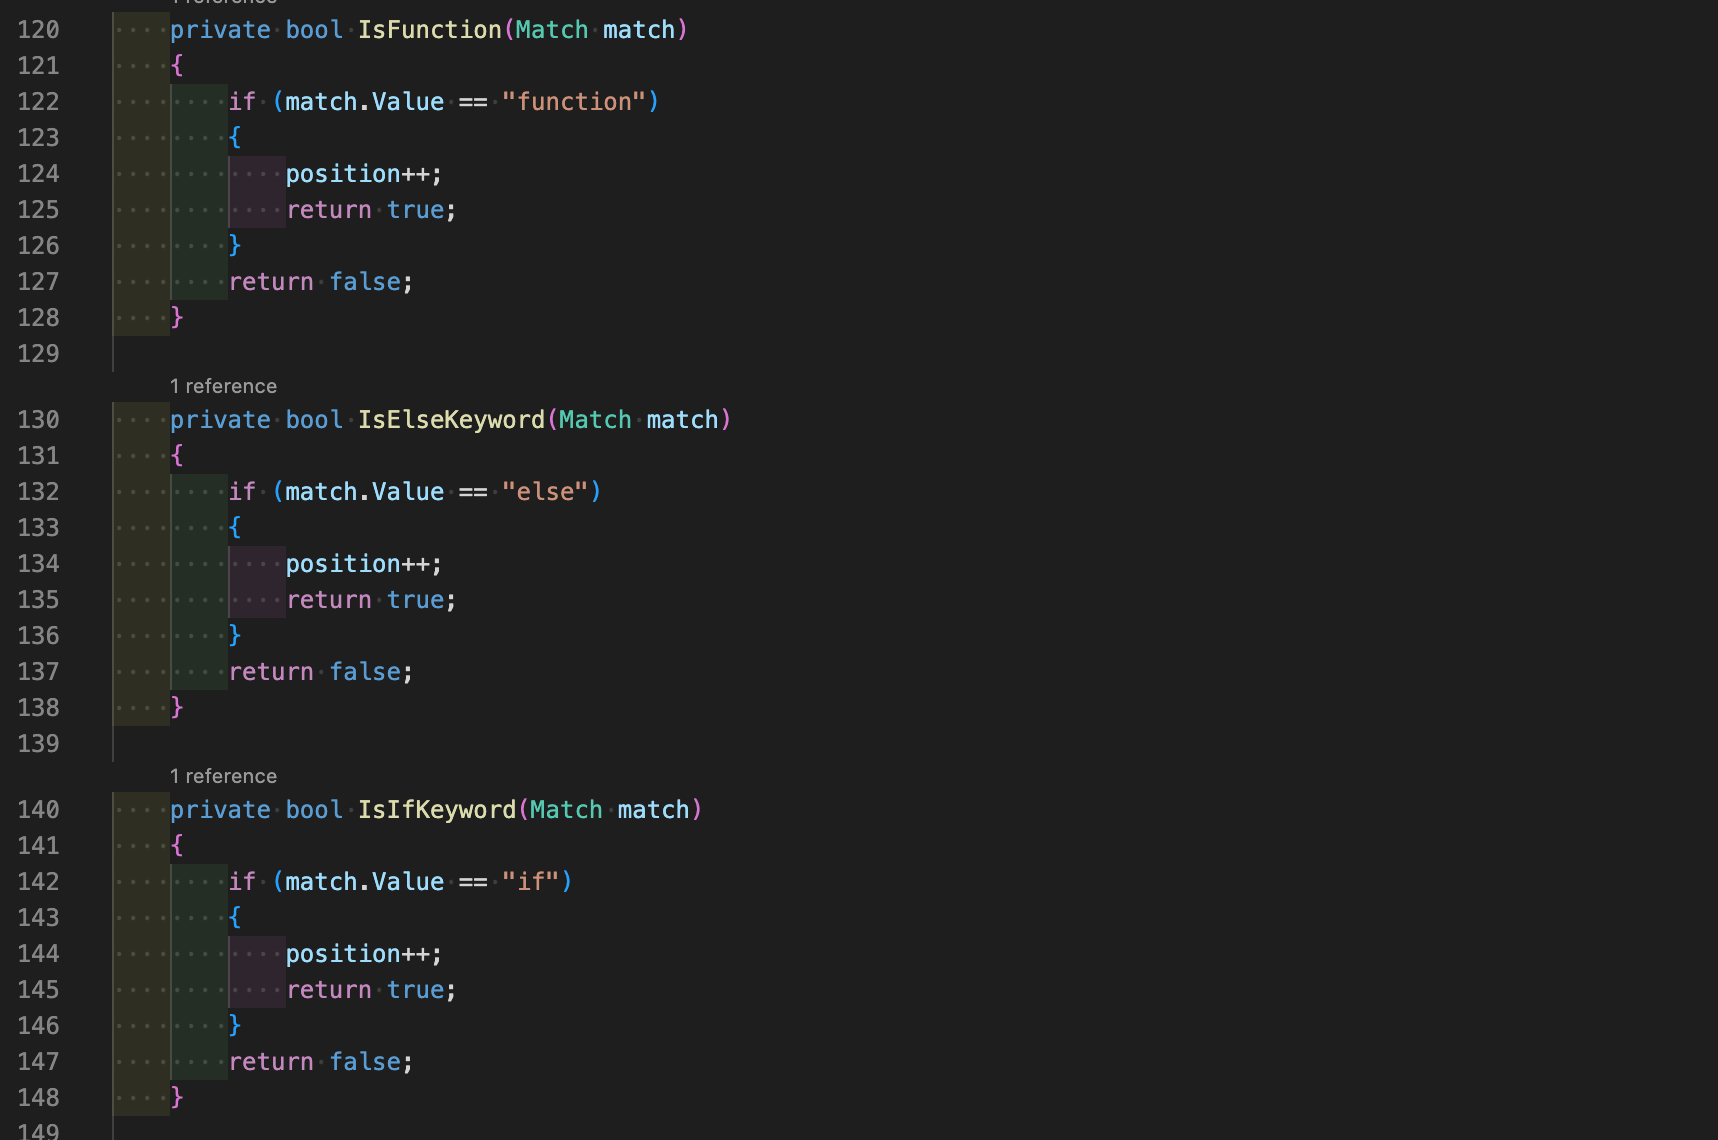
\includegraphics[width=6cm]{Pictures For Hulk/Figure3.png}
    \caption{Asignando mas tipos de tokens}
    \label{fig:logo}
\end{figure}

\subsection*{\tt Parser}
\addcontentsline{toc}{subsection}{Parser}

Cuando acaba el proceso de lexing, debemos parsear dichos tokens a ver si cumplen con la gramatica del programa.

En este proyecto se usara la tecnica de Parsing descendente recursivo.

El parsing descendente recursivo es un método utilizado en el análisis sintáctico de un lenguaje de programación. Consiste en construir un árbol sintáctico a partir de una cadena de entrada, aplicando reglas de producción de manera recursiva desde la raíz hacia las hojas del árbol.

El proceso de parsing (análisis sintáctico) se basa en una gramática formal que describe la estructura sintáctica del lenguaje. Esta gramática se representa mediante reglas de producción en forma de BNF (Backus-Naur Form) o alguna otra notación similar.

El análisis sintáctico descendente recursivo se inicia con un símbolo inicial de la gramática y recorre la cadena de entrada de izquierda a derecha. A medida que avanza, va aplicando las reglas de producción correspondientes para construir el árbol sintáctico. El proceso es recursivo porque cada regla de producción puede invocar a otras reglas de producción, de manera que se van explorando todas las posibles combinaciones de derivaciones hasta llegar a las hojas del árbol.

En general, cada no terminal de la gramática se asocia a una función o método en el código del parser, y la llamada a dicha función representa la aplicación de una regla de producción. Estas funciones se llaman recursivamente unas a otras para construir el árbol sintáctico.

Luego es pasado al evaluador donde se evalua cada nodo del arbol y se da una respuesta al input.

\end{document}